\chapter{Cluster Shape Encoding}
In this chapter my work will be discussed. First there will be a description of the data format, the cluster of pixels, analysing its properties and the reason behind the encoding. Then, a detailed description of the methods implemented will follow. Finally, the test of such methods will be reported.
\section{Cluster of Pixels}
\label{sec:cluster}
As said in chapter 3, the sensors of ITS-Upgrade are characterized by a binary readout and therefore only the information that can be obtained is whether or not a particle was crossing the pixel. Pixels in which the collected charge coming from the ionization exceeds a defined threshold are called \textit{fired pixels}. When a charged particle passes through a sensor, it loses energy in a region whose dimension depends on the parameters of the particle itself, such as its energy and the impact angle. Therefore, normally, it fires a set of adjacent pixels.\\
%
\begin{figure}
  \centering
  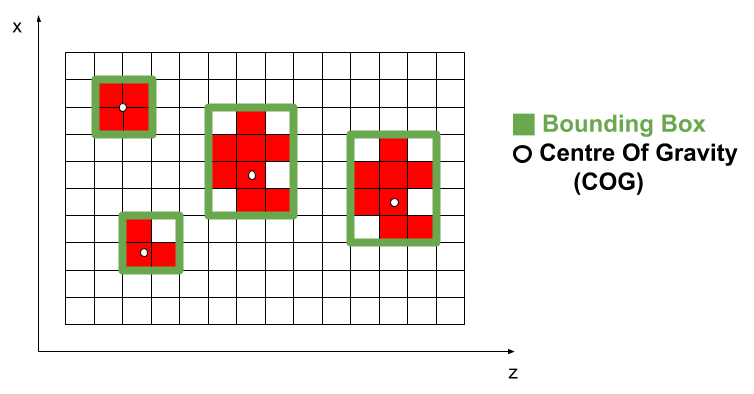
\includegraphics[scale=0.55]{figures/cluster.png}
  \caption{Example of different clusters on the same sensor. All the clusters have different positions, but two of them have the same shape.}
  \label{fig:clusters}
\end{figure}
%
A set of adjacent fired pixels forms a \textit{cluster}. Clusters are the data elements of the ITS and are used for the reconstruction of the trajectories of the charged particles which generated them. An example of clusters can be seen in Figure \ref{fig:clusters}. Each cluster in its raw format contains different kinds of information, which depend only on geometrical aspects. Each cluster has a particular shape, a specific pattern of fired pixels, which along my work is called \textit{topology}. As shown in Figure \ref{fig:clusters}, different clusters can have the same topology.\\
Some characteristics are shared by clusters with the same topology. For example, the dimensions of the \textit{bounding box}, which is the smallest rectangle that can entirely contain the cluster, are clearly the same for all the clusters with the same shape. A second common piece of information is the position of the \textit{centre of gravity} (COG) of the topology within the bounding box, since this position is uniquely determined by the disposition of the fired pixels. The position of the COG is extremely important, since it is assumed to be the most probable impact position of the particle that generated the cluster. The uncertainty related to this quantity, which will be discussed later, is also the same for all the clusters with the same topology. The position of the cluster within the sensor is, instead, different from cluster to cluster. It is expressed as the coordinate of a reference pixel of the cluster within the matrix described by the pixels of the chip, in the form (\textit{row}, \textit{column}). The reference pixel of a cluster is defined as the pixel containing the COG of the cluster. This information is then converted into a physical length by a simple product of the coordinates by the pitch of the pixel. Each sensor has its own local frame, where z is the beam direction, x is orthogonal to z and lies on the surface of the sensor, y is orthogonal to the x-z plane, forming a right-handed Cartesian system. The passage from the local to the global frame is then performed during the reconstruction of the tracks, using matrices implemented in AliRoot.\\
In the next section, the storage of the cluster data will be described, explaining the reasons behind this work.
\section{Data Compression}
The data size is an extremely important factor to hold in consideration during the design of a detector. The ALICE experiment, for example, has been designed for the study of heavy-ion collisions, with the necessity to identify all the particles produced in such collisions and to reconstruct their trajectories. This leads to the generation of a huge data volume. As mentioned in section \ref{datavol}, after the trigger selection, the data rate of all the detectors can reach 25 GB/s, while the physic content of many events could be small, with a DAQ archiving rate of about 1 GB/s. It is therefore clear that online processing is necessary to compress data avoiding the loss of physics content. The data rate will increase significantly after the upgrade, principally because of the increased collision rate. In particular, the data rate of all the detectors is estimated to be $\sim$ 1 TB/s \cite{o2}, where almost 1 TB/s is given by the TPC. For the ITS the data rate will increase both for the higher collision rate and because of the higher number of readout channels ($\sim 10^{10}$). In particular, it is expected to increase to $\sim$ 40 GB/s, more than the current data rate of the whole ALICE apparatus. The data reduction starts immediately after the cluster-funding process through the compression with the Huffman coding, which will be shortly described in the next section. With Huffman compression it is possible to reduce the data size of a factor that depends on the the noise occupancy: in the worst case scenario, with many noisy pixels, data size is reduced to  $\sim$ 26 GB/s, while in case of low noise it is reduced to $\sim$ 4.3 GB/s \cite{o2}.
\subsection{Huffman Coding}
\label{sec:huff}
Huffman coding is one of the most used lossless data compression algorithms, based on the relative frequency of the elements constituting a file. Huffman maps an element (for example a character in a text file) into a bit sequence of variable length according to its frequency: the most frequent element is mapped into the shortest string. The result is a Huffman table, of which an example is given in Table\ref{tab:huff}. It is the Huffman table corresponding to the sentence ``\textit{Trentatrè trentini entrarono in Trento, tutti trentatrè trotterellando.}'': the most frequent character (t) is mapped into a two-bit sequence, while the least common ones are mapped in the longest bit strings. In this way it is possible to contain the information of the sentence in a shorter bit string. The size of the original file is 72 B, but after compression it becomes 30 B, more than a factor 2 of compression. This example is trivial, but it allows to understand the utility of Huffman compression when applied to big files. Indeed, the most frequent character is encoded as the shortest bit string, therefore every time this character appears it is substituted by the corresponding Huffman code: the shortest string appears the highest number of times, allowing to save much storage space. Moreover, the less the frequency distribution of the elements is uniform, the more storage space is saved, since the most common character, hence the shortest bit string, appears much more often than the least common ones. This saving is obtained at the cost of creating a Huffman table and consulting it during the compression and the decompression processes, operations which are time consuming. For this reason, if the compression/decompression time is an important factor, it is necessary to pay attention to the number of entries in the table, since the former is proportional to the latter \cite{huffman}.
%
\begin{table}
\centering
 \begin{tabular}{|c|c|c|}
  \hline
  Character & Frequency & Huffman code\\
  \hline
  t & 15 & 01 \\
  r & 10 & 110 \\
  n & 9 & 101 \\
  e & 7 & 000 \\
  \_ & 7 & 001\\
  o & 5 & 1001 \\
  i & 4 & 11111 \\
  a & 3 & 11110 \\
  è & 2 & 10000 \\
  l & 2 & 10001 \\
  T & 2 & 111011 \\
  u & 1 & 111010 \\
  , & 1 & 111001 \\
  . & 1 & 111000 \\
  \hline
 \end{tabular}
 \caption{Huffman table related to the sentence ``\textit{Trentatrè trentini entrarono in Trento, tutti trentatrè trotterellando.}''.}
 \label{tab:huff}
\end{table}
%
\section{Cluster Data Encoding}
Every cluster is identified by its position and its topology. In section \ref{sec:cluster} it was said that the position of the cluster can be expressed as the coordinates of the reference pixel of the cluster within the sensor. This information must be combined with an identifier of the chip, whose position in the experiment frame is known. It is possible to store the position of the reference pixel not as its absolute raw number, but as the difference between its row number and that of the previous stored pixel. With the study of the frequency distributions of these differences, it is possible to see that they are not uniform and consequently it is possible to benefit from this non uniformity using Huffman coding. Similarly, the identifiers of the chips can be stored as the difference between the identifier of the chip which is being analysed and the previous one. Its distribution is not uniform as well and this element can be compressed using Huffman too. Both these distributions are strongly dependent on the occupancy in the detector. For this reason, it is possible to use different Huffman tables according to the multiplicity. In particular the multiplicity can be binned and for each multiplicity bin a Huffman table is defined. This information, together with the topology, defines the cluster data:
\begin{displaymath}
\begin{split}
  \mathrm{MultID[\textcolor{red}{\Delta ChipID_1}(\textcolor{Cerulean}{Col}, \textcolor{LimeGreen}{\Delta Row}, \textcolor{Plum}{Patt})_1 \  ... \ (\textcolor{Cerulean}{Col}, \textcolor{LimeGreen}{\Delta Row}, \textcolor{Plum}{Patt})_n \textcolor{SkyBlue}{\Delta EndChip}] }\\
 \mathrm{[\textcolor{red}{\Delta ChipID_2}(\textcolor{Cerulean}{Col}, \textcolor{LimeGreen}{\Delta Row}, \textcolor{Plum}{Patt})_1 \  ... \ (\textcolor{Cerulean}{Col}, \textcolor{LimeGreen}{\Delta Row}, \textcolor{Plum}{Patt})_n \textcolor{SkyBlue}{\Delta EndChip}]\ ...}
 \end{split}
\end{displaymath}
\textit{MultID} is the multiplicity bin, used to pick up the appropriate Huffman table to encode/decode the information about the row number and the identifier of the chip; \textit{$\Delta$ChipID} is the difference between the identifier of the cluster being analysed and the previous one; \textit{Col} is the column number of the reference pixel; \textit{$\Delta$Row} is the difference between the row number of the reference pixel of the current cluster and the previous one. \textit{EndChip} is a special identifier that flags the end of the chip. \textit{Patt} is instead the information related to the topology, which will be discussed in the next section.
\section{Cluster Topology Encoding}
The cluster topology, in its raw format, consists of a sequence of bits whose length depends on the number of pixels within the bounding box: a fired pixel is represented by a 1, while an off pixel by a 0. Such a string can become very long for large clusters and consequently storing the information about the cluster topology as the complete bit-mask would require the usage of much storage space.
%
\begin{figure}
  \centering
  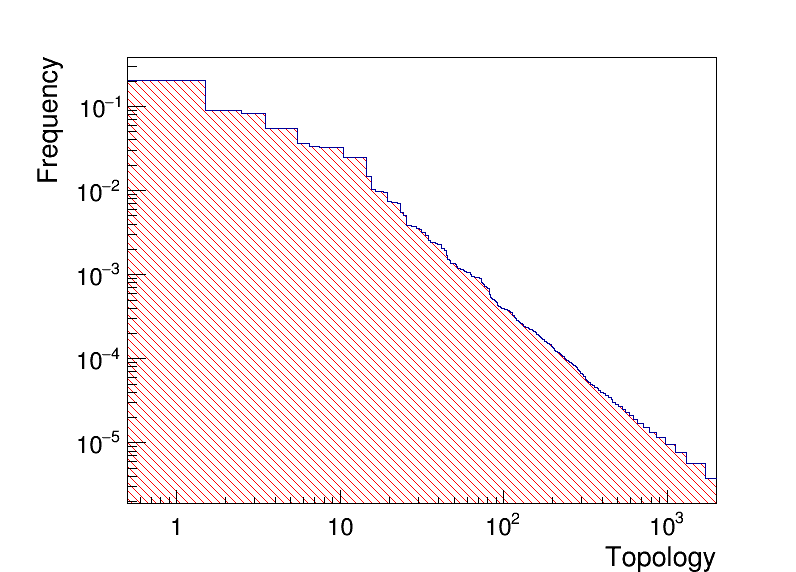
\includegraphics[scale=0.5]{figures/ciccio.png}
  \caption{Frequency distribution of the topologies obtained through a Monte Carlo simulation of 20 Pb-Pb events.}
  \label{fig:topdistro}
\end{figure}
%
This issue can be solved by creating a dictionary containing all the topologies. In this way it is possible to store a reference to an entry of the dictionary instead of the complete bit-mask. Since a reference is an integer, its length is fixed. In Figure \ref{fig:topdistro} a frequency distribution of the topologies, obtained simulating 20 minimum-bias Pb-Pb events, is reported. This distribution is highly non uniform and consequently the compression via Huffman would be extremely convenient in terms of storage space. However, due to the high number of different elements, the processes of compression and decompression become inefficient. Therefore, there is the necessity to reduce the number of entries in the dictionary and this can be done by grouping rare topologies, whose frequency is under a defined threshold, under a common reference.\\
In the next sections, the steps needed for the construction of the dictionary of the topologies will be described and a detailed description about the method of grouping will be given.
\section{Software Development}
The objective of this work is the implementation of some software for the construction of the dictionary described above and for the realisation of the related mechanisms of matching between the cluster topology and the corresponding entry in the dictionary. In particular this software will be used online, during the data acquisition in Run3. It must not be developed to work in AliRoot or ROOT environment: the two data analysis frameworks contain many features that are not necessary during the data acquisition and therefore the machines used for online operations have nor AliRoot and ROOT installed. For this reason several C++ classes, which can be used on every machine with a C++ compiler installed, have been implemented:
\begin{itemize}
 \item \textbf{MinimTopology} is a support class which contains the whole information necessary to characterize a topology;
 \item \textbf{Dictionary} is the proper dictionary, containing the information about all the common topologies and the groups of rare topologies;
 \item \textbf{BuildDictionary} is the class dedicated to the construction of the dictionary starting from the data;
 \item \textbf{LookUp} is used to match online the topology of clusters with the corresponding entry in the dictionary;
 \item \textbf{FastSimulation} can simulate a population of topologies with a frequency distribution determined by the dictionary. 
\end{itemize}
\section{Uniqueness of the Keys in the Dictionary: Hash Functions}
The dictionary must fulfill a few requirements. First of all, each entry in the dictionary must be uniquely identified by a key. The key must have specific characteristics: it must have a defined length, which must be the same for each entry of the dictionary, and it must be comparable with the other keys, in order to be sortable. Typically in a database the key is an integer, since such a type has the needed characteristics. Unfortunately, the topology is a bit string whose length is determined by the size of the bounding box and it cannot be used as a key. It is necessary to convert the topology as a string of variable length into a string of defined length. This operation is performed using a \textit{hash function}, which is a function that maps data of arbitrary size into data of fixed size. In particular, in this work a C++ implementation of the function MurmurHash2 is used. The name suggests its working principle: it is the combination of the words multiply (Mu) and rotate (r). MurmurHash2 processes the input string four bytes at a time, performing bitwise and multiplication operations, and combines all the four-byte chunks to give as a result a four-byte sequence. The choice of MurmurHash2 was made considering its characteristics: it has a good uniformity of the output distribution and it is fast if compared with other algorithms \cite{hash}. Indeed, the hash function must be as fast as possible, since it must be used online. The uniformity of the output instead is related to the non injectivity of the hash function: while the input of the hash function can be any string of bits, the output must be a positive integer (four-byte sequence) and therefore can be each integer in the range [0, 2$^{32}$ - 1]. If the distribution of the outputs is uniform, it is more likely that two different input strings are mapped into two different integers. Unfortunately, even if the MurmurHash2 function has a good uniformity, it is not injective: in very rare cases (< 1/1000) two different strings are mapped into the same hashcode. All the classes must be solved to use the dictionary. This operation is done in the class \textit{MinimTopology}, which will be described in the next section.
%
\begin{figure}
  \centering
  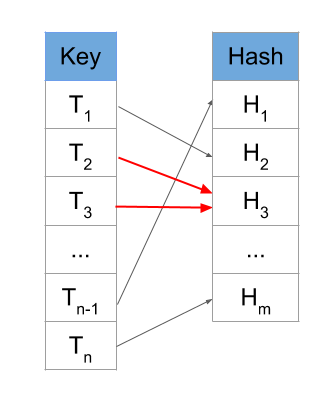
\includegraphics[scale=0.5]{figures/clash.png}
  \caption{Example of clash: MurmurHash2 maps two topologies (T$_2$ and T$_3$) into the same hashcode (H$_3$).}
  \label{fig:clash}
\end{figure}
%
\section{Class MinimTopology}
The class MinimTopology is the basis of this work since it is used by all the other classes. This class contains the information necessary to characterize a topology: the pattern, in string format, and the corresponding hashcode, generated from the pattern with a method that will be described soon. Starting from the pattern, the only sequence of bits is not enough to identify it uniquely. For example, the sequence 1111 could represent four fired pixels in a raw, or four fire pixels in a column, or a square of four pixels, all fired. Beside this information also the dimensions of the bounding box are needed. In this way it is possible to correctly interpret the sequence of pixels that constitutes the pattern. An example of pattern encoding within the class MinimTopology is given in Figure \ref{fig:pattern}. This topology has three rows and three columns, corresponding to a sequence of nine pixels. The pattern is encoded in a string where the first two bytes are respectively the number of rows and the number of columns. The remaining bytes of the string are used to encode the proper pattern, i.e. the sequence of pixels that constitutes the topology itself. In the example the pattern consists of nine pixels, therefore two bytes are necessary, since a byte is made of 8 bits. A 1 is associated to each fired pixel, a 0 to each off one. From this string a four-byte hashcode is generated using MurmurHash2, but at this stage it is possible that two different patterns are mapped into the same 4-byte sequence. There is therefore the necessity to solve the clashes. One method could be to mark with a flag the entries of the dictionary for which there is a clash and then proceed with the direct comparison between the patterns until the ambiguity is erased. However, this method require additional operations. It is first necessary to check whether the hashcode is marked with a clash-flag (even if there are not collisions) and then to resolve the ambiguities through a direct comparison. In fact there is a method to avoid the useless operation of the flag check: it is possible to use a eight-byte hashcode, in which the first four bytes are the usual four-byte hashcodes previously described and the last four bytes are the first four bytes which constitutes the pattern (the bytes starting from the third one of the string). In this way when two eight-byte hashcodes are compared, a comparison of both the hash generated with MurmurHash2 and the first thirty-two pixels is performed. Therefore, in case two different topologies are mapped into the same four-byte sequence by the hash function, the clash is solved at the same time of the four-byte hashcode comparison.
\begin{figure}
  \centering
  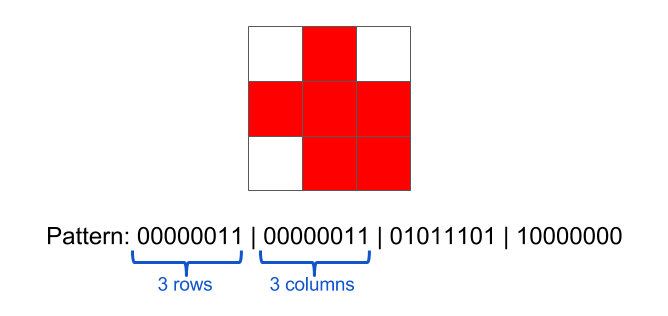
\includegraphics[scale=0.5]{figures/pattern.png}
  \caption{Example of pattern encoding: the first two bytes are respectively the number of rows and the number of columns; the remaining bytes are the pattern itself.}
  \label{fig:pattern}
\end{figure}
%
Summing up, the class MinimTopology has two data members:
\begin{enumerate}
 \item a string in which the pattern of pixels is stored;
 \item a eight-byte hashcode, generated from the pattern with the method just described, which uniquely identifies the topology.
\end{enumerate}
%
\section{Reduction of the Entries of the Dictionary: Grouping}
\label{sec:group}
The second requirement for the dictionary concerns the number of entries. As said in section \ref{sec:huff}, the Huffman becomes inefficient when the number of different elements (in this case the number of topologies within the dictionary) is high. For this reason there is the necessity to limit the number of entries of the dictionary to at most O(10$^3$). This objective is achieved by grouping rare topologies under a common reference, called \textit{GroupID}. The groups must be formed to gather rare topologies with similar characteristics, i.e. with similar errors related to the estimated impact position of the particle that generated the cluster. The grouping is necessarily a lossy operation, since the information about the pattern of pixels, and therefore about the position of the impact point of the single rare topology, is lost in favour of average quantities. However, this loss is bearable, since it concerns rare topologies and therefore it interests a very small fraction of the data.\\
The chosen grouping criterium concerns the dimensions of the bounding box: it is based on the assumption that topologies with similar dimensions have similar uncertainties related to the impact point position. As it will be seen later, for each common topology the uncertainty on the impact point position derives from the distribution of the impact points themselves (or rather their first reconstruction) with respect to the COG position. In the case of groups of rare topologies this method is not applicable, since in different topologies the position of the COG within the bounding box can be extremely different and the distribution of the impact points (their first reconstruction) can be different too. Since it is not possible to rely on these distributions, the error is evaluated with a method that takes into account the worst situation: the position of the impact point is assumed to be equally probable in the whole area of the bounding box. The error associated to the position of the COG is therefore that of a uniform distribution. In particular, a uniform distribution in the range of x(z) dimension of the bounding box:
\begin{equation}
 \sigma_x \; = \; \frac{N_{rows} \cdot d_x}{\sqrt{12}} \ \ \ \ \  \sigma_z \; = \; \frac{N_{columns} \cdot d_z}{\sqrt{12}}
\end{equation}
where $d_x$ and $d_y$ are respectively the pitch of the pixel along x and z directions.
Considering a uniform distribution the error might be a bit overestimated, but it is important to consider that this approximation involves rare topologies and hence a very small fraction of the data.\\
The grouping is based on a two-dimensional binning: a rare topology is assigned to a particular group according to its number of columns and rows. An example of grouping can be seen in Figure \ref{fig:gruppi}. The two rare topologies in the figure have very different patterns, but they have have a similar number of rows and columns (in this case exactly the same) and are mapped to the same group. The position of the COG in the bounding box is very different between two topologies, but after the grouping this information is lost. What remains is the position of the pixel containing the COG, which is the reference pixel of the cluster. Its centre is considered as the best estimate of the impact point of the particle. The error associated to the hit-point position is that of an uniform distribution, as just described. In this way, with a loss of detail on a small fraction of the total data, it is possible to reduce the number of entries of the dictionary.
%
\begin{figure}
  \centering
  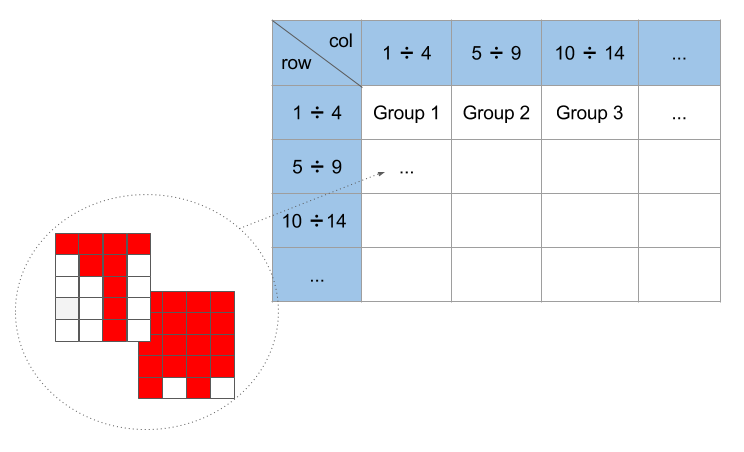
\includegraphics[scale=0.5]{figures/gruppi.png}
  \caption{Example of grouping: the two rare topologies have the same number of rows and columns and belong to the same group.}
  \label{fig:gruppi}
\end{figure}
%
\section{Class Dictionary}
\label{sec:dic}
In this section the structure of the class \textit{Dictionary}, the central class of the developed software, will be described. In order to understand the reasons behind the design of the class, it is necessary to analyse the lookup mechanism, represented in Figure \ref{fig:lucap}. During the data acquisition, it is necessary to associate to each cluster the corresponding entry within the dictionary in real time. From the cluster in its row data format, using the class \textit{MinimTopology} an eight-byte hashcode is generated from the pattern in string format. The hashcode uniquely identifies a specific topology, common or rare.
Common topologies must have their own entry in the dictionary, while rare topologies are referred to an entry that corresponds to a group of rare topologies with similar characteristics (previous section).
Therefore it must be possible to discern common topologies from rare topologies in such a way that, when a hashcode is generated, its corresponding key can be either found in the dictionary, if the hashcode belongs to a common topology, or is given after computing its group membership. Therefore, two elements are needed in the dictionary:
\begin{enumerate}
 \item a list containing the whole needed information about common topologies and group of rare topologies;
%  \item a structure containing all the relations between the hashcodes of the common topologies and the groupIDs in the list.
\end{enumerate}
%
\begin{figure}
  \centering
  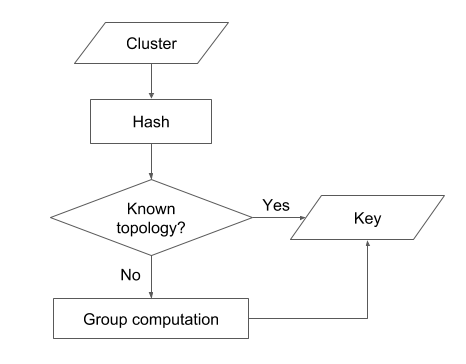
\includegraphics[scale=0.6]{figures/lucap.png}
  \caption{Scheme of the lookup mechanism.}
  \label{fig:lucap}
\end{figure}
%
\subsection{Vector of Groups}
The first element of the dictionary is a list containing the information about common topologies and groups of rare topologies. From now on the word ``group'' will be used also for common topologies, which constitutes a group of only one element. Hence the term \textit{groupID} means both the identifier of a group of rare topologies and the identifier of a single common topology, interpreted as a group made of a single element. The list consists of a \textit{vector}, object of the C++ standard template library. Vectors are similar to arrays, since they use a continuous storage location for their elements, which can be directly accessed using pointers to elements as efficiently as in arrays. The advantage lies in their dynamic size, automatically changed during storage operations \cite{vector}. This functionality is exactly what is needed in this case, since the number of groups is not known a priori.\\
The vector contains one element for each group and the corresponding position is its groupID: at position 0 there is the element corresponding to the group whose groupID is 0, at position 1 groupID 1, and so on. Each element is a structure containing the information necessary to define the group:
\begin{enumerate}[a)]
 \item the position of the COG with respect to the centre of the reference pixel;
 \item uncertainties on the impact point position;
 \item upper limit of the cumulative frequency of the group.
\end{enumerate}
As far as the first point is concerned, there is a difference between common topologies and groups of rare topologies. In every case the reference pixel is defined as the pixel containing the COG, therefore this information is the distance between the COG and the centre of the pixel in which it lies. For common topologies this quantity allows to have a better estimate of the position of the impact point, since in many cases the COG does not coincide with the centre of a pixel. This kind of information is not available for groups of rare topologies, since the distance between the COG and the centre of the pixel can differ in each case, and hence it must be set to zero, being shared among all the topologies within the group. However, considering that the uncertainties related to the position of the impact point are considered in the worst case scenario, i.e. those of an uniform distribution, and that this approximation concerns rare topologies, this partial loss of information does not significantly affect the precision of the data.\\
The uncertainties on the impact point position, along x and z directions, for common topologies are determined directly from the data. They are the standard deviations of the population of residuals (distance between the hit-point and the centre of gravity) respectively along x and z directions. It can sound strange to use the distribution of the distances between the COG and the hit-point positions, since the latter is the quantity that has to be determined. In fact, a rough estimation of the hit-point position is given during the first track reconstruction, which occurs online: this quantity can be used to determine the distribution of the residuals to have an estimation of the distance between the two points. A further description concerning the determination of the parameters of the distribution will be given later.\\
Finally, there is the information related to the cumulative frequency. The common topologies are sorted in descending order of frequency inside the vector. After the last common topology, there are the entries corresponding to the groups of rare topologies. For each entry the cumulative frequency is the sum of the frequencies of all the entries from the first to the one considered. The use of these quantities will be clear in section \ref{sec:fast}.
%
\begin{table}
\centering
\renewcommand\arraystretch{1.5}
 \begin{tabular}{|c|c|c|c|c|c|}
  \hline
  GroupID & d$_x$(COG,ref) & d$_z$(COG,ref) & $\sigma_x$ & $\sigma_z$ & Frequency\\
  \hline
  0 & d$_{x0}$ & d$_{z0}$ & $\sigma_{x0}$ & $\sigma_{z0}$ & f$_0$\\
  1 & d$_{x1}$ & d$_{z1}$ & $\sigma_{x1}$ & $\sigma_{z1}$ & f$_0$ + f$_1$\\
  2 & d$_{x2}$ & d$_{z2}$ & $\sigma_{x2}$ & $\sigma_{z2}$ & f$_0$ + f$_1$ + f$_2$\\
  ... & ... & ... & ... & .... & ... \\
  k & d$_{xk}$ & d$_{zk}$ & $\sigma_{xk}$ & $\sigma_{zk}$ & $\sum_{i=0}^{k} f_i$ \\
  k + 1 & 0 & 0 & $\sigma_{x(k+1)}$ & $\sigma_{z(k+1)}$ & $\sum_{i=0}^{k+1} f_i$\\
  k + 2 & 0 & 0 & $\sigma_{x(k+2)}$ & $\sigma_{z(k+2)}$ & $\sum_{i=0}^{k+2} f_i$\\
  ... & ... & ... & ... & ... & ...\\
  k + l & 0 & 0 & $\sigma_{x(k+l)}$ & $\sigma_{z(k+l)}$ & $\sum_{i=0}^{k+l} f_i$\\
  \hline
 \end{tabular}
 \caption{Example of a vector in a dictionary with $k$ common topologies and $l$ groups of rare topologies.}
 \label{tab:vec}
\end{table}
%
\subsection{Map}
\label{sec:map}
The second element of the dictionary is a map, which associates the hashcodes of the common topologies to their corresponding groupID. A map is an object of the C++ standard template library, in particular it is an associative array, i.e. a container in which the elements are stored as a combination of a \textit{key value} and \textit{mapped value}\cite{map}. In this case, the hashcode is the key value, unique for each topology, while the groupID is the mapped value. Each pair in the dictionary is uniquely identified by its key value and all the pairs are sorted in descending order with respect to the key value itself. A map is a balanced binary search tree, a data structure optimized for the lookup, the addition and the removal of an item. In particular, the complexity of both the insertion and the lookup is $O(\log(n))$, that means that the average number of operations needed for the insertion of a new item or for looking up a key in the structure scales with the logarithm of the number of entries. These characteristics make the operation of lookup fast and this is exactly what is needed to match online a topology with the corresponding entry in the dictionary. Moreover, there is another property that makes a map appreciable, i.e. the \textit{insert} method. This method is used for the insertion of an element, which is uniquely identified by its key: one key cannot appear twice in the map. If one tries to add to the map an element identified by a key that is still not present, this is added in a certain position according to its key value. Otherwise, if the key has already been inserted in the map, the insert method returns an iterator to the element identified by that particular key value, which is therefore easily accessible and prone to be modified. This feature is extremely useful during the construction of the dictionary and represents a further reason for the use of a map.\\
Summing up, in the dictionary the map is used to have a fast match between the hashcode of a common topology and the corresponding groupID.
%
\begin{table}
\centering
\renewcommand\arraystretch{1.5}
 \begin{tabular}{|c|c|}
  \hline
  Hashcode & GroupID\\
  \hline
  H$_0$ & gr$_{\pi_{0}}$\\
  H$_1$ & gr$_{\pi_{1}}$\\
  H$_2$ & gr$_{\pi_{2}}$\\
  ... & ...\\
  H$_{k-1}$ & gr$_{\pi_{k-1}}$\\
  H$_k$ & gr$_{\pi_{k}}$\\
  \hline
 \end{tabular}
 \caption{Example of a vector in a dictionary with $k$ common topologies.\\ ($\pi_0$, ... , $\pi_k$) are the permutations of the integers in the range [0 ; k].}
 \label{tab:map}
\end{table}
%
\section{Class BuildDictionary}
The class \textit{BuildDictionary} is used for the construction of the dictionary from the data. It is necessary to make few important considerations about this point. First, it is necessary to devote some data for building a dictionary of topologies: these data will not be available for physics measurements, but their sacrifice is necessary to save storage space for the upcoming events. Since Pb-Pb collisions are extremely precious for the ALICE experiment, pp collisions are likely to be used. Second, but not for importance, the population of topologies is strongly dependent on the parameters of the detector, like, for example, the threshold. Every time one parameter is changed a new dictionary must be built, since a completely different population of topologies is obtained.\\
The construction of the dictionary is articulated in two steps:
\begin{enumerate}
 \item inclusion of the information of new topologies;
 \item elaboration and finalisation of the dictionary;
\end{enumerate}
These two steps will be separately described in the next sections, focusing on the methods and the attributes necessary for the execution of the process.
\subsection{Inclusion of the Information of New Topologies}
In this step the data necessary for the construction of the dictionary are collected. There is the necessity of a temporary structure in which it is possible to store the information about the already met topologies: this structure is a map, where the key values are the hashes of the topologies.  A map has been chosen for the insertion properties described in section \ref{sec:map}: when a new topology is processed, the related eight-byte hashcode is generated. If it is not present in the temporary structure, a new item corresponding to the topology is added. If the topology has already been met, then an iterator to the corresponding element of the map is returned and the record can be easily updated with the new information. In the temporary map the key value is the hash, while the mapped value is a structure which contains all the important quantities of the topology:
\begin{itemize}
 \item number of occurrences;
 \item dimensions of the bounding box, x and z directions;
 \item distance between the centre of gravity and the centre of the pixel, along x and z directions;
 \item mean value of the distribution of the residuals, x and z directions;
 \item variance of the distribution of the residuals, x and z directions.
\end{itemize}
The insertion of a new element, or the update of an element already present, is performed by the method \textit{AccountTopology}. A scheme about the working principle of AccountTopology can be found in Figure \ref{fig:account}. This method takes as arguments the pattern of the cluster in string format and the residuals along x and z directions. Starting from the pattern in string format, it  generates the unique hashcode and then tries to insert the entry in the temporary map. In case of first insertion the record is created: its number of occurrences is set to 1 and the geometrical properties, such as the dimensions of the bounding box or the position of the COG, which are the same for all the clusters with the same topology, are consequently set. As far as the parameters of the residual distributions are concerned, the mean value is set to the value of the residual itself and the variance is set to zero, since it is the first element. In case of update, the process is a bit different. The geometrical properties do not need to be updated, being the same for all the clusters with the same topology. The number of occurrences is clearly incremented by one. The update of the parameters of the residual distributions is more tricky. Indeed, since this software must be able to be executed on machines on which ROOT is not installed, functionalities such as histograms are not available. Moreover the implementation of such a feature is out of discussion, since it would take quite a lot of storage space and the insertion of an element would require a certain number of operations, that means computing time.
Instead, both the mean values and the variances of the distributions are directly updated using the respective online algorithms:
\begin{equation}
 \overline{x}_{n + 1} \; = \; \frac{n \cdot \overline{x}_n + x}{n + 1}
\end{equation}
\begin{equation}
 \sigma^2_{n + 1} \; = \; \frac{n \cdot \sigma^2_n + (x - \overline{x}_n)(x - \overline{x}_{n + 1})}{n + 1}
\end{equation}
In this way, it is possible to obtain the parameters of distribution avoiding to store the information of each element of the topology population. On the contrary, for each distribution it is sufficient to store two float numbers, i.e. eight bytes each.\\
This process of collection of new data continues until enough statistics is collected. Then, the dictionary can be elaborated and finalised.\\
%
\begin{figure}
  \centering
  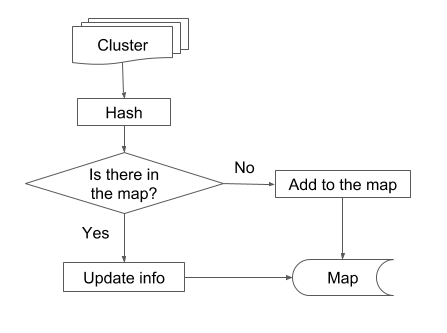
\includegraphics[scale=0.6]{figures/account.png}
  \caption{Scheme of AccountTopology method: the temporary information about the collected topologies is update with the information of a new element.}
  \label{fig:account}
\end{figure}
%
\subsection{Elaboration and Finalisation of the dictionary}
Once all the needed data have been collected, it is possible to start building the dictionary. It is first necessary to define the number of common topologies: this operation is done considering the frequencies of the topologies collected during the fist step. Common topologies are those whose frequency is above the frequency threshold (the definition of the threshold will be discussed later in this section). In order to establish which topologies are common, it is necessary to sort the elements in the temporary map in descending order of frequency. However, this operation cannot directly be done with the temporary map, since it is already ordered with respect to the key values. Hence, a support data structure is needed. A vector is used for this purpose: each element of the vector is a pair, corresponding to a particular topology, where the first member is the frequency and the second is the hashcode. The elements of the vector are taken directly from the temporary map and then are sorted in descending order with respect to the frequency. In this way, it forms a list of hashcodes, each corresponding to a particular topology among those collected in the previous step, sorted from the most to the least frequent. The order of the vector brings some benefits to the analysis of the collected topologies and the consequent construction of the dictionary. Indeed, once the first element below the threshold is found, all the following ones are for sure rare topologies as well and therefore they belong to groups. A scheme about the processing of the data in the temporary map can be found in Figure \ref{fig:build}.
Starting from the most frequent topology, when a common topology is processed, its important information are stored in the dictionary, both in the map and in the vector. In particular, the pair hashcode-groupID is inserted in the map. It is important to remember that a common topology is a group made of one only topology and, therefore, the groupID coincides with the position of the topology inside the vector member of the dictionary. Then, the important information about the groups is inserted in the vector of the dictionary: the position of the COG with respect to the centre of the reference pixel, the uncertainties on the impact point position, the cumulative frequency. For all the common topologies this operation is repeated exactly in the same way. When the first topology below the frequency threshold is found, the map inside the dictionary is completed, since it concerns exclusively common topologies. At this point the vector must be filled with the information about the groups. The most of the needed quantities are known a priori: the position of the COG, which for groups is set to zero, and the error related to the impact position, which depends only on the dimensions of the bounding box. The cumulative frequency, instead, must be computed, summing the frequencies of all the topologies belonging to the same group. After this piece of information is added to the vector, the dictionary is completed and can be stored in a binary file. In the next section the determination of the frequency threshold will be described.
%
\begin{figure}
  \centering
  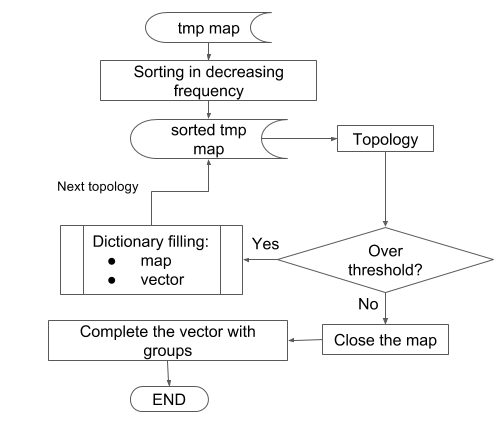
\includegraphics[scale=0.6]{figures/build.png}
  \caption{Scheme of the elaboration and finalisation of the dictionary.}
  \label{fig:build}
\end{figure}
%
\subsection{Setting of the Frequency Threshold}
\label{sec:thr}
The frequency threshold can be set in three ways. The first method is the direct definition: the threshold is directly set to a particular value. All the topologies with a frequency below this value are considered rare and therefore belong to groups. For example, if the threshold is set 10$^{-5}$, then all the topologies with a frequency below 10$^{-5}$ are inside groups. The second method is the cumulative definition: a threshold for the cumulative frequency of the common topologies is set so that the least frequent common topology has a cumulative frequency below the defined threshold. For example, one assumes that the cumulative frequency threshold is set to 0.99999 (it is important to remember that the topologies inside the vector are sorted in descending order of frequency). For each element of the vector, the frequency must be summed with those of all the previous elements. Once this value exceeds the cumulative threshold, 0.99999, all the previous topologies are common, while the remaining ones are rare. Finally there is the definition of the number of common topologies: the number of common topologies is fixed and all the other ones are rare and hence inside groups.
\section{Class LookUp}
The class \textit{LookUp} is used during the data acquisition to match the topologies of cluster data to the corresponding entry of the dictionary. Since it is used online, it must be as fast as possible. The lookup mechanism is shown in Figure \ref{fig:lucap} and has already been mentioned in section \ref{sec:dic}. However, in this section it can be described more in detail thanks to the knowledge of the structure of the class Dictionary. When a cluster is processed, from the topology the corresponding hashcode is generated. Then, it is looked up in the map of the dictionary, which relates the hashcodes of common topologies with their groupID, i.e. their position inside the vector member of the dictionary. This operation is performed using the \textit{find} method of a map. In case the hashcode is found in the map, i.e. it belongs to a common topology, an iterator to the element is returned and therefore the corresponding groupID is given. Otherwise, if the hashcode is not found, i.e. it belongs to a rare topology, an iterator to the end of the map is returned. In this case, the groupID must be directly computed by the dimensions of the bounding box of the topology, using the two-dimensional binning described in section \ref{sec:group}.
\section{Class FastSimulation}
\label{sec:fast}
The class FastSimulation uses the information about the cumulative frequency to simulate a population of topologies with the same frequency distribution of the data from which the dictionary was generated. It is fast because it allows to pass directly from the hit to the recpoint, i.e. impact point position with related uncertainties, avoiding to simulate the production of the signal inside the sensor. The working principle is extremely simple. A random number in the range [0; 1] is generated using the Mersenne-twister engine of the C++ standard template library, which is based on the Mersenne-twister algorithm for the generation of pseudorandom numbers \cite{mersenne}. Then, the function \textit{upper\_bound} is used on the vector member of the dictionary, with the random number as argument: this function returns an iterator to the first element of the vector that compares greater than the argument. From the iterator, the groupID is then obtained. In this way the probability to obtain a particular groupID is proportional to its frequency. It is important to notice that for rare topologies it is not possible to reproduce the information about the particular instance inside the group, but just the average information about the group itself, since only this is recorded. The fast simulation is important because it allows to simulate a final output of the detector that reproduces that of the real data, avoiding to simulate all the process of signal generation and reconstruction that can introduce error and generate a difference between the real final output and the simulated one. 
%
\section{Test on simulated data}
This section focuses on the tests of the algorithms above described on simulated data. The simulations are performed in AliRoot environment, where the particles produced in heavy-ion collisions are created using HIJING and PYTHIA generator, after setting up the initial conditions of the interaction, such as the energy in the frame of the centre of mass and the range of variability of the impact parameter. For minimum bias events, i.e. without any kind of restrictions, the range is set to 0 < b < 14 fm. For central events, instead, the impact parameter range is 0 < b < 2 fm. After the generation step, the particles are transported through the detector using the software GEANT3. Then, the response of the detector and the consequent signal generation are simulated by dedicated algorithms present in AliRoot. Similarly, the event reconstruction is performed with dedicated tools present in AliRoot. The sensors considered in this simulations are note those that will be used during the data acquisition, since the final sensor (ALPIDE, section \ref{sec:alpide}) is still under development and the Monte Carlo for simulating the response of such a sensor is under development as well. The simulations are based on a prototype of MIMOSA (\textit{Minimum Ionizing MOS Active pixel sensor}), a monolithic pixel sensor that has been developed in parallel to ALPIDE but then abandoned in favour of the latter. The response of the sensor, of course, is not the same as ALPIDE, but the output has the same characteristic non-uniformity on which this work is based.\\ 
%
\begin{figure}
  \centering
  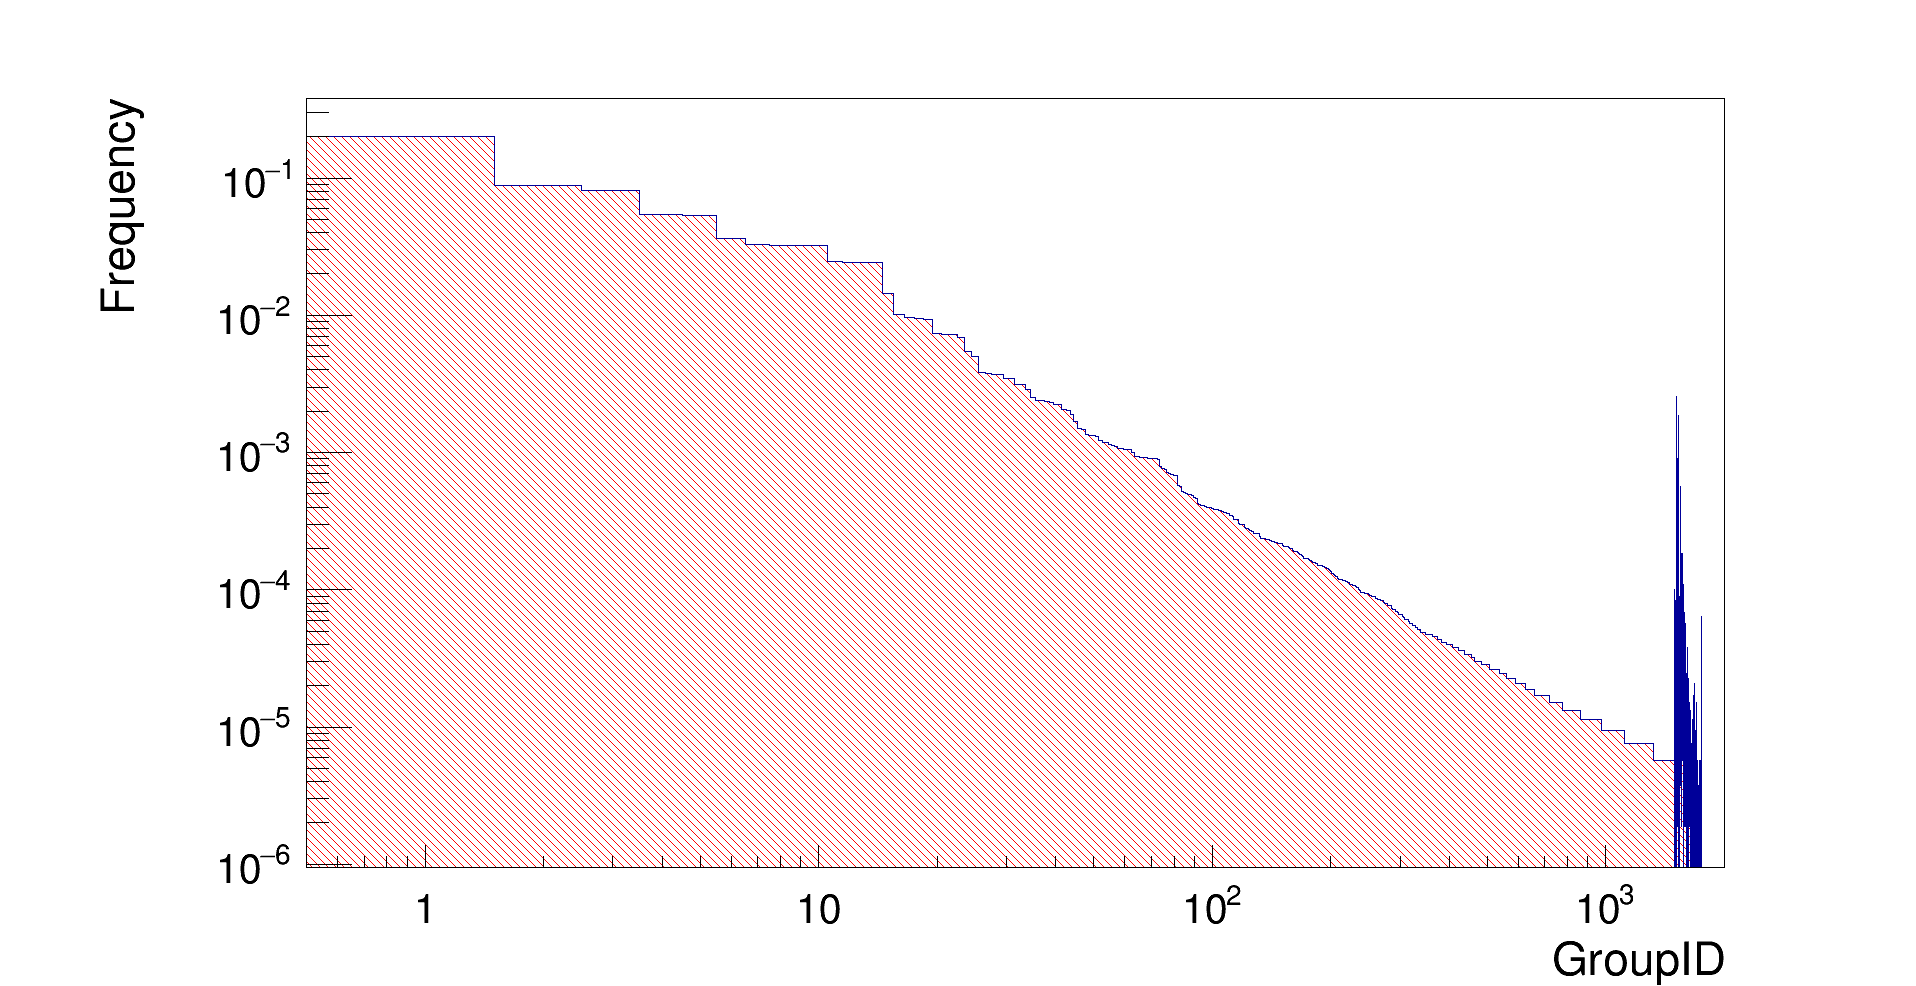
\includegraphics[scale=0.2]{figures/grouped.png}
  \caption{GroupID distribution corresponding to twenty minimum bias events. It is possible to see a tail corresponding to the groups of rare topologies.}
  \label{fig:groupdistr}
  \vspace{1.5cm}
  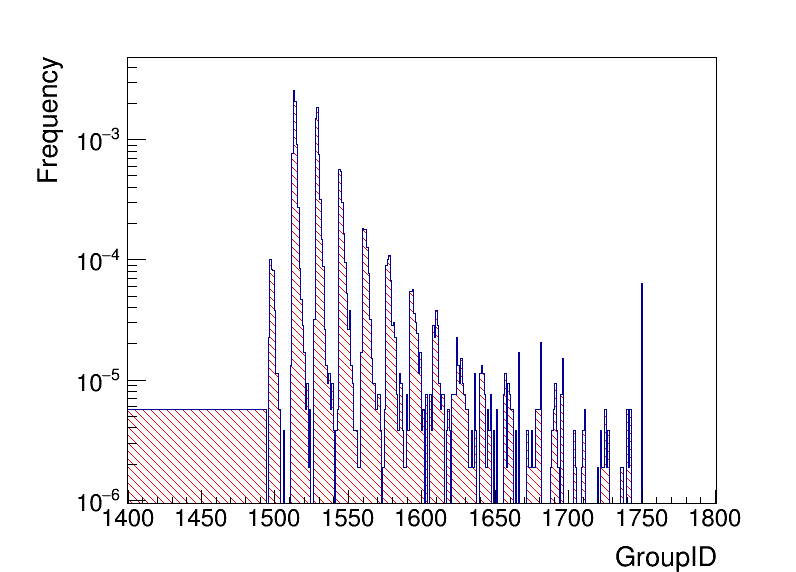
\includegraphics[scale=0.45]{figures/zoom.png}
  \caption{Zoom on the tail of the distribution of the groupIDs in Figure \ref{fig:groupdistr}, corresponding to the groups of rare topologies.}
  \label{fig:groupzoom}
\end{figure}
%
In Figure \ref{fig:groupdistr} the distribution of the groupIDs of a population of topologies corresponding to twenty minimum bias events is reported. As one could expect, it is very similar to the distribution of the topologies reported in Figure \ref{fig:topdistro}, remembering that each common topology defines a group made of a single element. The only difference is that the topologies under the frequency threshold have been grouped. In particular, in this example the number of groups has been directly fixed with the method described in section \ref{sec:thr}. The frequency distribution of the topologies, before the grouping operation occurs, is monotonically decreasing. After the definition of the threshold, the rare topologies are grouped according to the dimensions of their bounding box and the information about the corresponding groupIDs are queued to the dictionary and it appears as a spike in the tail of the groupID distribution. The grouping is done via a two-dimensional binning in the dimensions of the bounding box, as described in \ref{sec:group}. Since the largest dimension of a cluster is 32$\times$32 pixels, both the row-span and the column span have been binned into sixteen bins of range 2. The number of rare topologies is 256 and with this granularity it is possible to obtain a good approximation on the uncertainties related to the estimated hit-positions. Indeed, if the bin range were bigger, topologies with different dimensions, hence with a different uncertainty on the hit-position, would form a unique group, with an excessive loss of detail. In Figure \ref{fig:groupzoom} a zoom on the tail of the frequency distribution, corresponding to the groups of rare topologies is reported, is reported. In such distribution a kind of pattern can be seen. It can be explained considering the way in which the rare topologies are grouped: first they are grouped in ascending order of row-span, then, for each row-span bin, in ascending order of column span. For this reason, since spikes becomes smaller when the groupID increases, rare topologies with a small row-span are more frequent than rare topologies with bigger dimensions. The last bin, instead, has more entries since it collects also those topologies whose dimensions exceed the cut-off value 32$\times$32 pixels.
\section{Benchmark of LookUp}
In this section the benchmark of the LookUp algorithm is described. This benchmark consists of the measurement of the time necessary to match a topology with the corresponding entry in the database. Since the time necessary to match a single topology is very small, of the order of few microseconds, it is not possible to measure it alone, due to the resolution of the internal clock of the CPU. For this reason, in this benchmark the time necessary to identify all the topologies produced in twenty minimum-bias Pb-Pb events is measured. These measurements depend on many aspects. First of all, they depend on the characteristics of the machine, as for instance the clock frequency of the processor or the size of the memory. Moreover, there are other factors to take into account, like the processes executed by the CPU in background, that affects the measurement and are not under the control of the user. For this reason, it is not possible to have precise timing of the algorithms, but it is however important to have an idea of the average time or at least of the order of magnitude. Even if not much precise, in this case it is important to have an idea of the process time, since it must be compatible with the data-acquisition rate foreseen for Run3. For this reason, this benchmark was done trying to average the effects that cannot be controlled.\\
All the topologies generated in the twenty minimum-bias Pb-Pb events are stored in a vector in the string-format previously described. The benchmark tool measures the time necessary to identify all the topologies within the vector: a stopwatch is started at the beginning of the operation of matching and stopped after the last element of the vector have been process. This operation is repeated one hundred times: the mean value is taken, with the RMS as uncertainty.
%
\begin{figure}
  \centering
  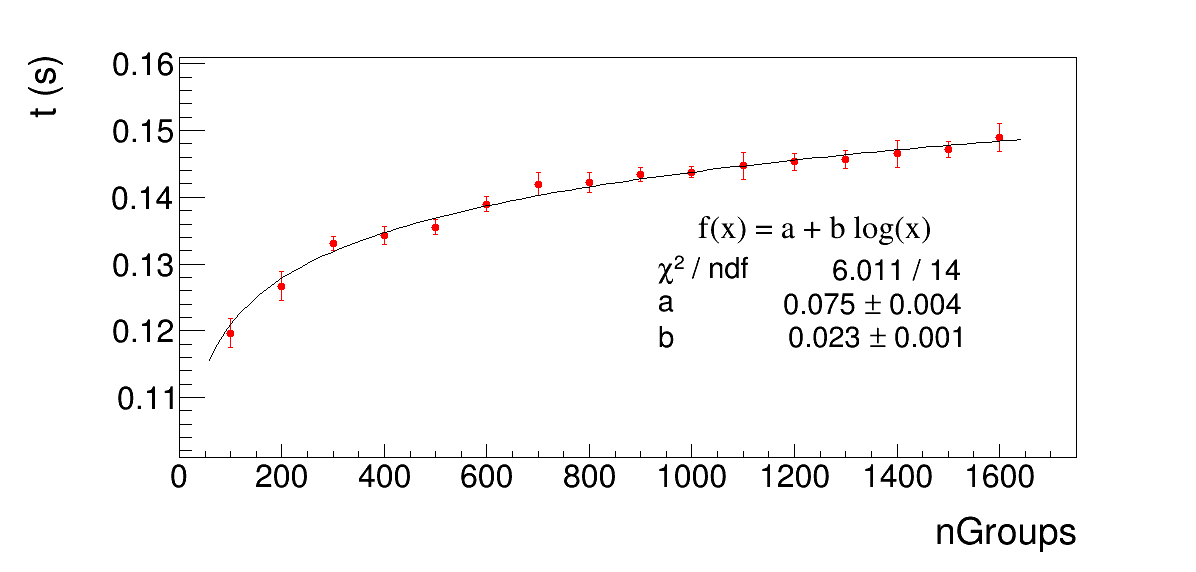
\includegraphics[scale=0.3]{figures/ordered.png}
  \caption{Benchmark of the LookUp algorithm as a function of the number of groups.}
  \label{fig:ordered}
  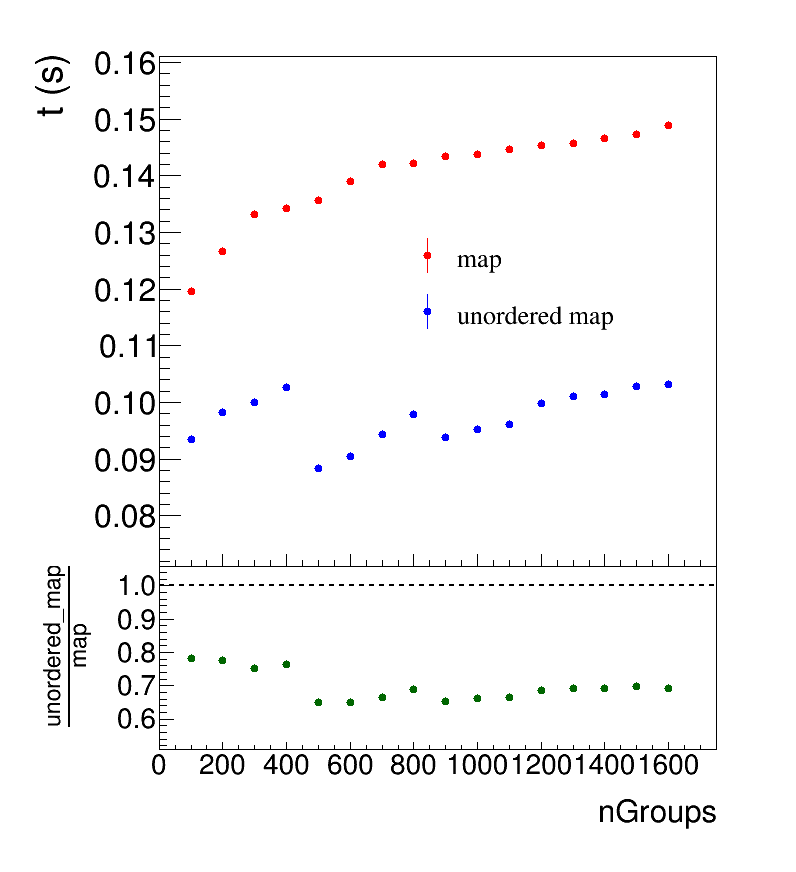
\includegraphics[scale=0.4]{figures/bench.png}
  \caption{Benchmark of the LookUp algorithm: the performances with a dictionary containing a map (ordered) are compared with those of a dictionary containing an unordered\_map. The comparison is made for dictionaries composed of a different number of groups. In the lower part, the ratio about the to methods is shown.}
  \label{fig:bench}
\end{figure}
%
This measurement is done for different numbers of groups within the dictionary: it is represented by the red points in Figure \ref{fig:ordered}. It is possible to see how the time necessary to process all the data increases with the number of groups, i.e. with the number of entries in the database. This trend is expected because the dictionary contains a map and the lookup time for a map on average scales with the number of entries as O($\log(n)$). The logarithmic scaling is also confirmed by $\chi^2$ test with a significance of the 5\%. The largest time measure is (0.149 $\pm$ 0.002) s. From this value it is possible to get a rough estimation of the average time necessary to process one event, dividing by the number of events, in this case twenty. The average time for processing one event is about 7.5 ms, corresponding to a rate of about 130 Hz. This value is well below the collision rate of 50 kHz foreseen after the upgrade. However, this process of topology identification can be done in parallel by many CPUs. A rough estimation of the necessary number of processor can be given dividing the collision rate by the process rate, obtaining that about 390 processors are needed. %This value is just an estimation, since it does not take into account the non parallelizable component of the process, due, for example, to the memory sharing.
\subsection{Implementation with unordered\_map}
It is possible to optimize the LookUp performances of the software using a very small change in the code, i.e. substituting anywhere \textit{map} with \textit{unordered\_map}. unordered\_map is a feature of C++11, the version of C++ language published in 2011. While a map is an ordered structure, based on binary tree, an unordered\_map, as its name suggests, is unordered and is based on a hash table, which is a standard of C++11, providing fast insertion, lookup and deletion. A benchmark on the modified software has been done on the same data on which the benchmark of the standard implementation has been done.
In Figure \ref{fig:bench} the results of this new benchmark are reported, compared with those of the old implementation. In particular, in the lower part the ratio between the times with the two methods is reported. The time necessary to identify a topology with the new method is from 20\% up to 35\% faster than with the previous method. The reason behind this improvement is the use of hash table, optimized in C++11. However, it is possible to notice a strange behaviour passing from 400 to 500 groups with the new method. These measurements have been repeated few times and on different computers with different characteristics, but each time the gap passing from 400 to 500 is present.The reason behind this strange behaviour is not clear: using diagnostic tools, as for example valgrind \cite{valgrind}, it is possible to see that with 500 groups some methods of the standard template library are called, which were not called with 400 groups. This could mean that there are some optimisation in the code of unordered\_map that occurs when the size of the structure exceeds a certain value. Understanding the reason of this behaviour is beyond the aim of this work, since it means to study how unordered\_map is implemented.\\
Also in this case an estimation of the time necessary to process a minimum-bias event can be given. The largest time measure is (0.103 $\pm$ 0.001) ms. The average time for processing one event is about 5.2 ms, corresponding to a rate of about 190 Hz. Dividing the interaction rate by the processing rate, an estimation of the number of processor necessary to identify all the topologies of the clusters generated in a minimum-bias event is about 260. Even if this is a rough estimation, it is clear that there is an improvement with respect to the previous implementation.